
    \begin{abstract_online}{Formulation and Implementation of General Topological Network Criteria for Exploring the Structures of Confined Ice}{%
        \underline{A. Goswami}, J. K. Singh}{%
        }{%
        Department of Chemical Engineering, IIT Kanpur, India}
    We present a family of general topological criteria, for the determination of structures of quasi-one-dimensional and quasi-two-dimensional ices [1]. Confined systems are characterized by a plethora of diverse ordered structures and interesting hydrogen-bond-networks (HBNs), distinct from those formed in the bulk. Our methodology has no a-priori assumptions, and can be used as an exploratory tool for probing confined ice structures. In our recipe, primitive rings are identified, and further, only connections corresponding to hydrogen bonds are permitted. Figure 1 compares the accuracy of our methodology with that of Voronoi tessellation, for flat Monolayer Square Ice (fMSI). The prism identification scheme developed identifies prismatic units, which are the building blocks of ice nanotubes (INTs). In addition, we formulate novel and intuitive order parameters based on our topological network criteria, which are able to qualitatively and accurately describe phase transitions. \par  \begin{center}  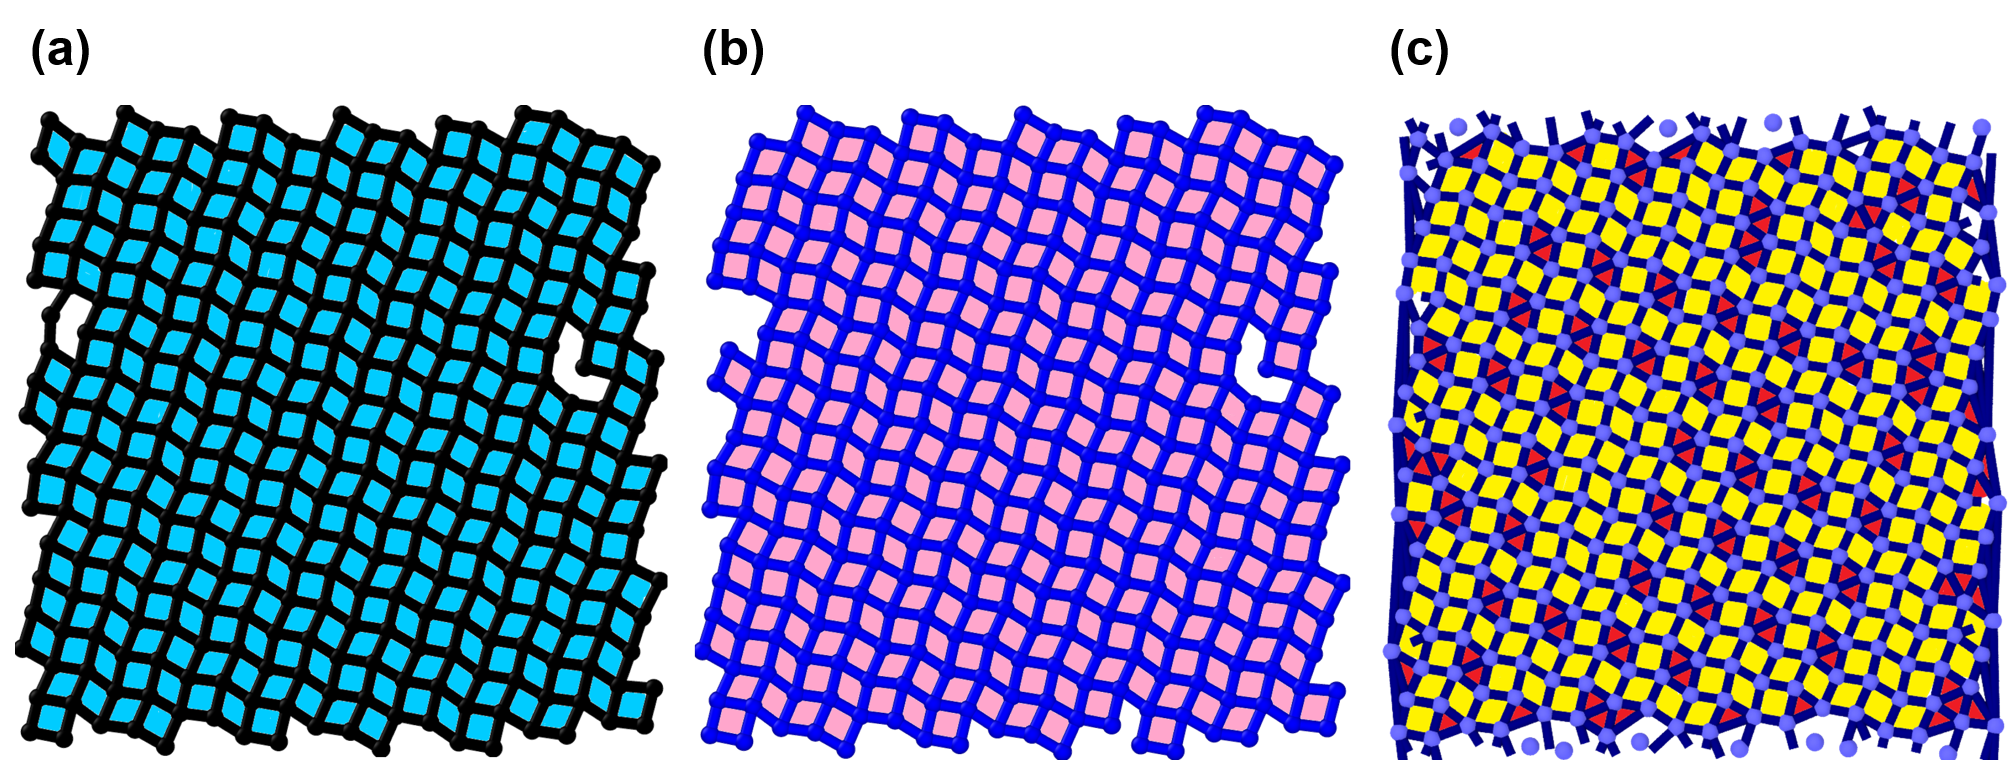
\includegraphics[width=0.8\linewidth]{abstracts/txt/figures/compareTopoVoro.png}  \caption{\textbf{Figure 1:} Comparison of the accuracy of Voronoi tessellation with our topological network criterion for identifying fMSI. fMSI is known to consist of 4-membered polygons. (a) The top view of the HBN, with 4-membered polygons shaded in cyan. Identification schemes should closely approximate the HBN connectivity. (b) The ring network generated by our topological network criterion, with 4-membered rings shaded in pink. (c) Neighbour bonds created by Voronoi tessellation. The bonds (in black) are generated by connecting neighbouring particles (blue) which share a Voronoi face. Polygons thus formed, with three and four edges, are coloured in red and yellow, respectively. The Voronoi cells are 5-membered and 4-membered polygons, depending on the coordination number.}  \end{center} We have subsumed this new methodology, along with other popular structure determination algorithms, into a framework developed for the analysis of molecular simulations. We present d-SEAMS (deferred Structural Elucidation Analysis of Molecular Simulations), a free and open-source post-processing engine [2]. The software automates the classification of ice structures for both confined and bulk ice for the first time. The framework of d-SEAMS is also unique, and designed to ensure reproducible research and easy extensions, without compromising functionality. D-SEAMS uses nix [3] for generating a reproducible and deterministic dependency build-graph, thus circumventing package dependency clashes [4]. A YAML-Lua scripting interface enables users to interact with the C++ backend. Figure 2 shows the work-flow implemented in d-SEAMS. Key features implemented include topological network criteria for bulk and confined ice, ring statistics, intuitive geometric order parameters and bond-orientational parameters. The outputs produced by d-SEAMS are consumable by popular graphics software suites, for immediate visual insights into the systems studied. \begin{center}  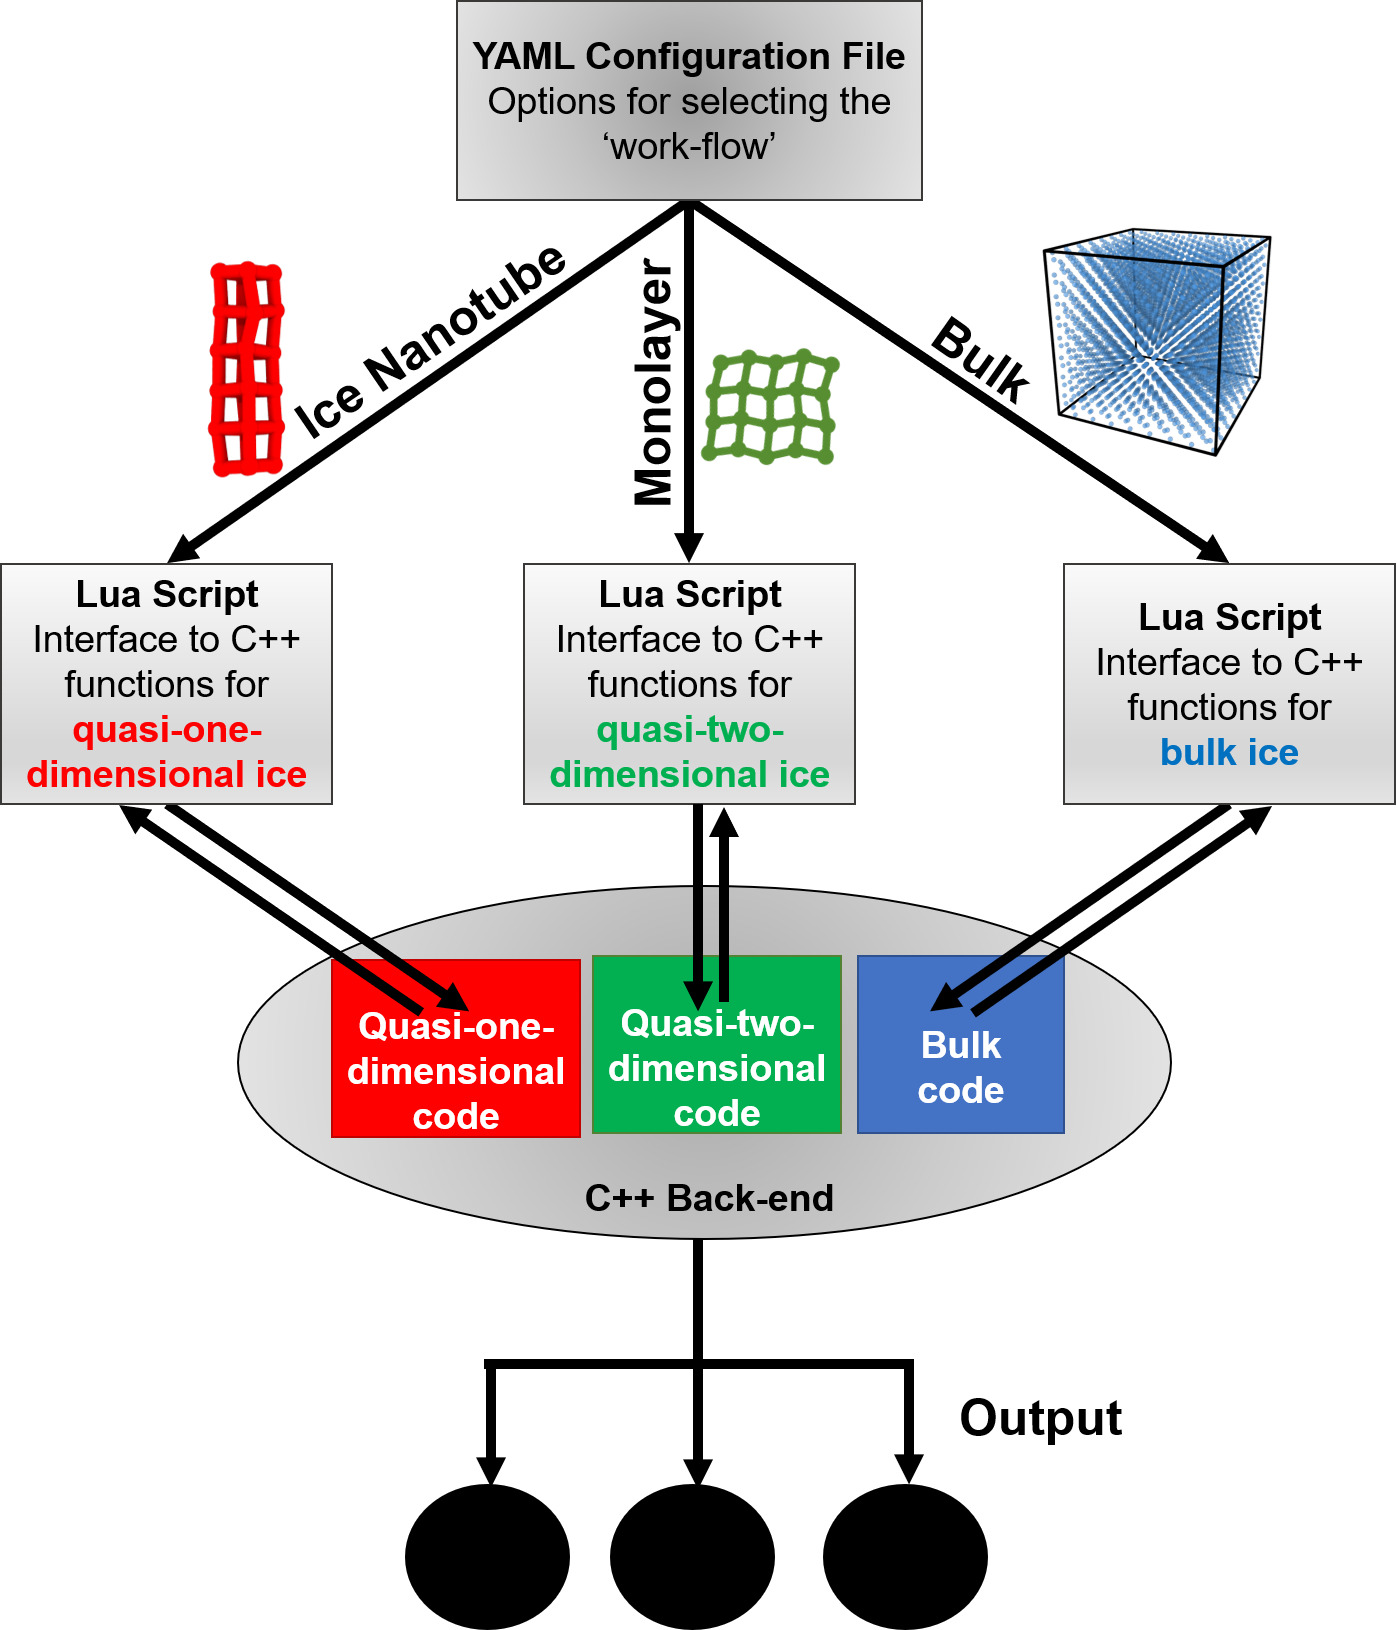
\includegraphics[scale = 0.4]{abstracts/txt/figures/workFlowChart.jpg}  \caption{\textbf{Figure 2:} Code pipeline of d-SEAMS. The YAML script file provides options to choose the  type of the system and the corresponding work-flow, for either bulk, quasi-one-dimensional  quasi-tqo-dimensional monolayer sytems. The Lua interface functions interact with the  C++ functions for each work-flow, and functions of other work-flows are not exposed to  the user.}  \end{center} 
    
        \textbf{References} \newline{}[1] Goswami, A., & Singh, J. K. (2020). A general topological network criterion for exploring the structure of icy nanoribbons and monolayers. Physical Chemistry Chemical Physics. doi:10.1039/c9cp04902a.\newline{}[2] Goswami, R., Goswami, A., & Singh, J. K. (2019). d-SEAMS: Deferred Structural Elucidation Analysis for Molecular Simulations. arXiv:1909.09830. (Submitted)\newline{}[3] Dolstra, E., Visser, E. Nix: A Safe and Policy-Free System for Software Deployment.\newline{}[4] Prins, J., Suresh, J., Dolstra, E. Nix fixes depency hell on all Linux distributions. Linux.\newline{}2008.
    \end{abstract_online}
    